\documentclass[MasterThesisMain.tex]{subfiles}
\begin{document}
\chapter{Theory}

\section{Electromagnetic Radiation}
	
\section{Fresnel equations for the ambient-substrate model}
When light is reflected upon a surface at an oblique angle, light is reflected and transmitted. Lights electric field is grouped into two oscillation directions which can be defined by two planes, the parallel plane p and the perpendicular plane s. The same applies for lights magnetic field. The parallel plane is defined by the incident and reflected light and the perpendicular plane is perpendicular to the parallel plane. Theory of light regards the two oscillation directions as the p-polarisation and s-polarisation.

Light is reflected and transmitted at the interface of the ambient and substrate\marginpar{Figure and model set up}. The boundary conditions at the interface for the electric and magnetic field\marginpar{Need to understand why B-field is true} in the p-polarisation can be written as:

\begin{align}
E_{i,p}\cos{(\theta_i)} &= E_{t,p}\cos{(\theta_t)} + E_{r,p}\cos{(\theta_r)}\\
\implies E_{t,p}\cos{(\theta_t)} &= E_{i,p}\cos{(\theta_i)} - E_{r,p}\cos{(\theta_r)}
\end{align} 

\begin{equation} 
B_{i,p} + B_{r,p} = B_{t,p}
\end{equation}

The subscripts of the electric and magnetic field denote the incident ray $i$, reflected ray $r$ and transmitted ray $t$ in the p-polarisation $p$ plane. The same boundary conditions for the s-polarisation can be expressed. This introduction to the fresnel equations will use the p-polarisation light. The boundary conditions of the magnetic field need to be reformulated to express the electric field, this is done in the following way. The Maxwell-Faraday equation and one dimension wave equations for the electric and magnetic field are expressed as:

\begin{equation}
\frac{\partial E}{\partial x} = - \frac{\partial B}{\partial t}
\end{equation}

\begin{align}
E = E_0 \cos{(Kx-\omega t)}\\
B = B_0 \cos{(Kx-\omega t)}
\end{align}

Using the Maxwell-Faraday equation the following equation can be formed:

\begin{align}
\frac{\partial E}{\partial x} &= - \frac{\partial B}{\partial t}\\
-K E_0 \sin{(Kx-\omega t)} &= -\omega B_0 \sin{(Kx-\omega t)}\\
E_0 &= \frac{\omega}{K} B_0\\
E_0 &= s B_0
\end{align} 

The constant $\frac{\omega}{K}$ is expressed as the speed $s$ of the light through a medium. In vacuum the speed is equal to the speed of light $s=c$, through a transparent medium the speed is equal to the speed of light divided by the refractive index of the medium $s =\frac{c}{n}$. The magnetic field boundary conditions can be expressed as:

\begin{align}
\frac{E_{i,p}}{s_i} + \frac{E_{i,p}}{s_i} &= \frac{E_{t,p}}{s_t}\\
\frac{n_i}{c}(E_{i,p}+E_{r,p}) &= \frac{n_t}{c}E_{t,p}\\
n_i(E_{i,p}+E_{r,p}) &= n_tE_{t,p}
\end{align} 

Though the law of reflection the angle of incident is also the angle of reflection $\theta_i=\theta_r$, placing this into the electric field boundary conditions, the electric field and magnetic field can be expressed as:

\begin{align}
(E_{i,p}-E_{r,p})\cos(\theta_i) &= E_{t,p}\cos(\theta_t) \label{eq:E}\\
\frac{n_i}{n_t}(E_{i,p}+E_{r,p}) &= E_{t,p} \label{eq:B}
\end{align}

Placing equation \ref{eq:B} into equation \ref{eq:E}, the amplitude reflectance coefficient and the reflectance can be calculated for the ambient-substrate system:

\begin{align}
E_{i,p}\cos(\theta_i)-E_{r,p}\cos(\theta_i) &= \frac{n_i}{n_t}(E_{i,p}+E_{r,p}) \cos(\theta_t) \\
E_{i,p}\cos(\theta_i) - \frac{n_i}{n_t}E_{i,p} \cos(\theta_t) &= \frac{n_i}{n_t}E_{r,p} \cos(\theta_t) + E_{r,p} \cos(\theta_i)\\
E_{i,p}(n_t\cos(\theta_i)-n_i\cos(\theta_t)) &= E_{r,p}(n_i\cos(\theta_t)+n_t\cos(\theta_i))\\
r_p = \frac{E_{r,p}}{E_{i,p}} &= \frac{n_t\cos(\theta_i)-n_i\cos(\theta_t)}{n_i\cos(\theta_t)+n_t\cos(\theta_i)}\\
R_p = \mid r_p \mid &^2 
\end{align}

The amplitude transmission coefficient and transmission can be equivalently formulated\marginpar{Complex refractive index fresnel eq can also be expressed}. 

\section{Fresenel equations for the ambient-thin film-substrate model}
The light reflecting and transmitting in this system will interfere both constructive and destructively. To model the optical interference, both the fresnel equation for reflection and transmission will be used:

\begin{align}
r_{jk,p} = \frac{N_k\cos(\theta_j)-N_j\cos(\theta_k)}{N_k\cos(\theta_j)+N_j\cos(\theta_k)} \quad r_{jk,s} = \frac{N_j\cos(\theta_j)-N_k\cos(\theta_k)}{N_j\cos(\theta_j)+N_k\cos(\theta_k)} \\
t_{jk,p} = \frac{2N_j\cos(\theta_j)}{N_k\cos(\theta_j)+N_j\cos(\theta_k)} \quad t_{jk,s} = \frac{2N_j\cos(\theta_j)}{N_j\cos(\theta_j)+N_k\cos(\theta_k)} 
\end{align}

The subscripts denote the reflection and transmission at definite interface. For example $r_{jk,p} = r_{01,p}$, denotes the reflection at the ambient-layer interface. In the ambient-thin film-substrate model, light at the ambient-thin film interface will be both reflected and transmitted into the layer. The transmitted ray will then be reflected and transmitted at the thin film-substrate interface. The reflected and transmitted phenomenon will proceed through out the thin film. The change in phase at the interface is given by $\exp(-i\beta)$. Figure \ref{fig:beta} represents the ambient-thin film-substrate model, this figure will be used to define the phase variation $\beta$.

The phase of the reflected ray will vary at the the ambient-thin film interface. This variation can be expressed as $K_0\bar{AD}$, where $K_0=\frac{2\pi n_o}{\lambda}$ is the propagation number in air. The phase variation of the transmitted ray is expressed as $K_1(\bar{AB} + \bar{BC})$, where $K_1=\frac{2\pi n_1}{\lambda}$, propagation number in the thin film. The length difference can be denoted as $\bar{AB} + \bar{BC} - \bar{AD}$, thus the phase variation of this length difference is:

\begin{equation}\label{eq:phasealpha}
\alpha = \frac{2\pi n_1}{\lambda}(\bar{AB} + \bar{BC}) - \frac{2\pi n_0}{\lambda}\bar{AD}
\end{equation}

Using snells law, $\bar{AD}=\bar{AC}\sin(\theta_0)$ and $\bar{AC}=2d\tan(\theta_1)$ as seen from figure \ref{fig:beta}, this reduces $\bar{AD}$ to:


\begin{align}
\sin(\theta_0) &= \frac{n_1}{n_0}\sin(\theta_1)\\
\bar{AD}&= 2d\frac{\sin(\theta_1)}{\cos(\theta_1)}\sin(\theta_0)\\
\implies \bar{AD}&= 2d\frac{\sin(\theta_1)^2}{\cos(\theta_1)}\frac{n_1}{n_0}
\end{align}

Inserting this into equation \ref{eq:phasealpha}
\begin{figure}
\centering
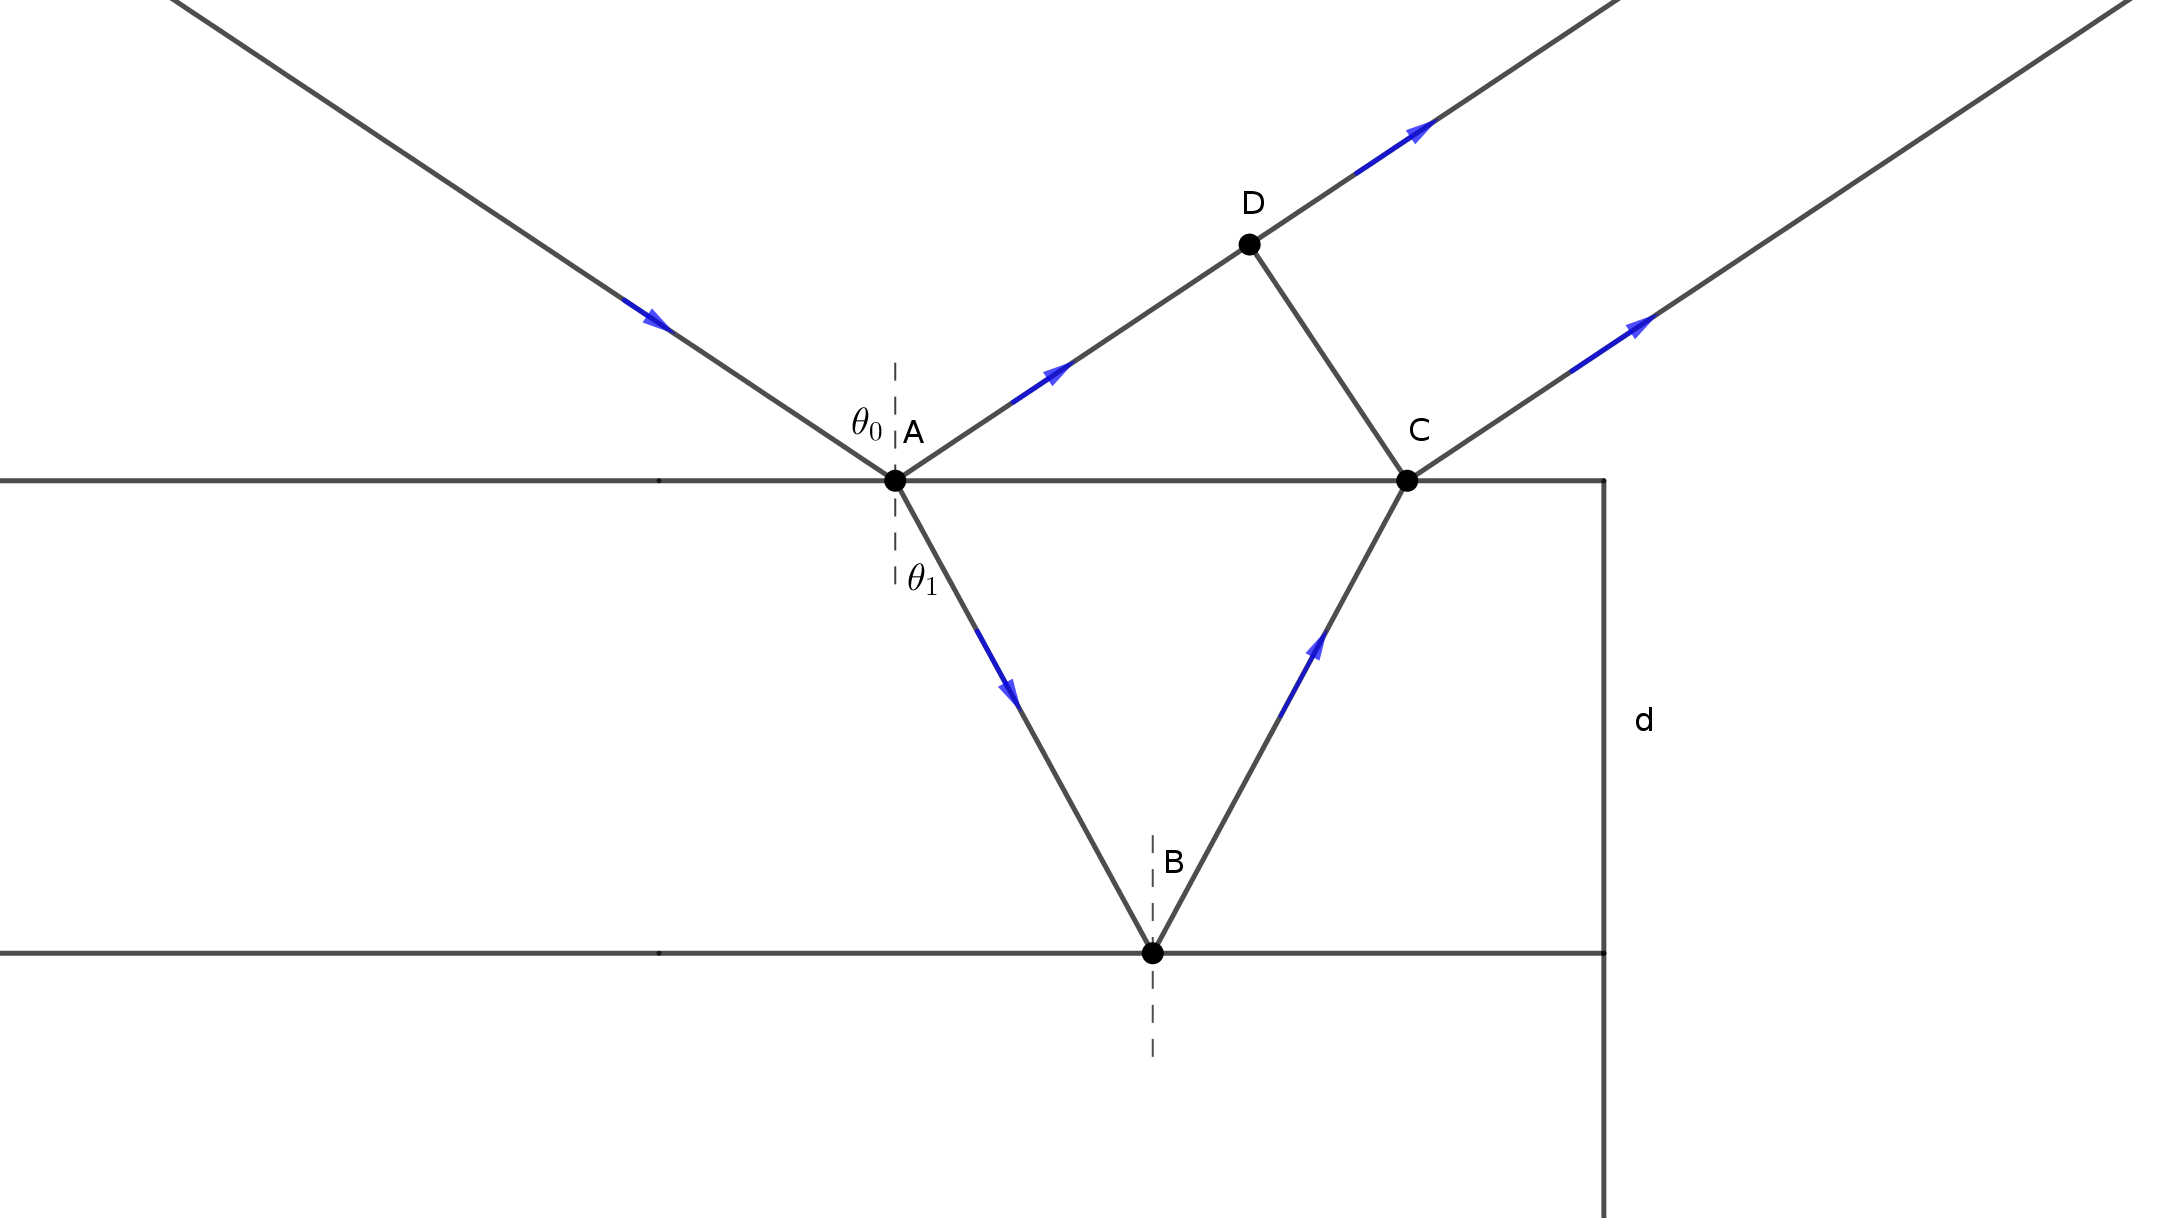
\includegraphics[width=\textwidth]{figbeta.png}
\caption{}
\label{fig:beta}
\end{figure}  
        
\end{document}